\documentclass[12pt]{report}

\usepackage[english]{babel}
\usepackage[utf8x]{inputenc}
\usepackage{geometry}
\geometry{a4paper}    

\usepackage{amsmath}
\usepackage{gensymb}
\usepackage{amssymb}
\usepackage{amsthm}
\usepackage{graphicx}
\usepackage{caption}
\usepackage{subcaption}
\DeclareMathOperator{\Tr}{Tr}
\usepackage[colorinlistoftodos]{todonotes}
\usepackage[toc,page]{appendix}
\usepackage{multirow}
\usepackage{float}
\usepackage{verbatimbox}
\usepackage[square,numbers]{natbib}
\usepackage{url}
\usepackage[framed]{mcode}
\usepackage{hyperref}
\usepackage{listings}
\usepackage{tcolorbox}

\tcbset{colback=blue!5!white,colframe=blue!50!black}

\def\*#1{\mathbf{#1}}

\linespread{1.5}

\title{MATLAB - An Introduction for Mathematicians}
\author{Scott Morgan, Alex Mackay \& Danny Groves}

\begin{document}
\maketitle

\section*{Introduction - The Matlab Interface}

\begin{itemize}
\item Matlab is a computational software package originally written by numerical analyst Clive Moler in the 1970s. 
\item Unlike other programming languages used in numerical computations like Fortran and C++, Matlab makes use of highly developed external libraries and functions which allows you to relieve yourself of many of the mundane tasks associated with programming. For example, Matlab has built in functions that can calculate matrix inverses, products and eigenvalues. All of these things would have to be hard-coded into a Fortran program, eating up time that could be spent on more important issues. 
\item With a very readable and easy to navigate interface, Matlab is a great starting tool for anyone interested in programming. 
\item Although it has many qualities, Matlab is not a perfect package for all computational tasks and what it gains in usability it loses on computational time. A program written in Fortran or C++ will run a lot faster in general than the same program written in Matlab, which may be of concern for very large programs. This, however, is most certainly \textit{not} of concern here, and all of the programs written in this course should take only a fraction of a second to run on a workstation.
\item It should be noted that these notes are designed only as a companion to the classes which they accompany - a student should not expect to gain any insight from these notes without attending class.
\item E-mail corrections and/or comments are always welcome and can be directed to \url{MorganSN@cardiff.ac.uk}
\end{itemize}


\subsection*{Installing Matlab}

\begin{itemize}
\item A student Matlab subscription is currently £29\footnote{Correct as of 19/07/2016} and is highly worth the spend. However, if you are currently a student at Cardiff then you can get the academic license key for installation on your home computer for free. The download and install process is described in detail on the Intranet at \\
\footnotesize \url{https://intranet.cardiff.ac.uk/students/support-and-services/technical-help-and-support/software-support/software-for-home-use/matlab} \\
\normalsize
Note that you will need to be logged into the Intranet to access this page. \\ 
There is also a thorough guide to installation from MathWorks, available at \\
\footnotesize \url{http://uk.mathworks.com/help/install/ug/install-mathworks-software.html} \normalsize
\item Alternatively, you can use Matlab at any of the workstations around the university, available through \textit{Cardiff Apps}, or you can use GNU Octave.
\item GNU Octave is free, open-source software which can run many Matlab commands. However, as with everything in life, you get what you pay for and thus, Octave can be buggy, slow and is lacking certain features that may make your life a misery.
\item Installing Octave on Windows can also be a pain, although it is described in detail on the web at \url{https://www.gnu.org/software/octave/download.html}.
\item Installing Octave on Ubuntu is easy and can be accomplished with
\begin{lstlisting}[language=bash]
  $ sudo add-apt-repository ppa:octave/stable
  $ sudo apt-get update
  $ sudo apt-get install octave
\end{lstlisting}
\end{itemize}

\subsection*{Using Matlab for the first time}

\begin{itemize}
\item On opening Matlab for the first time you should be presented with a window similar to this:
\begin{figure}[h]		
	\centering
	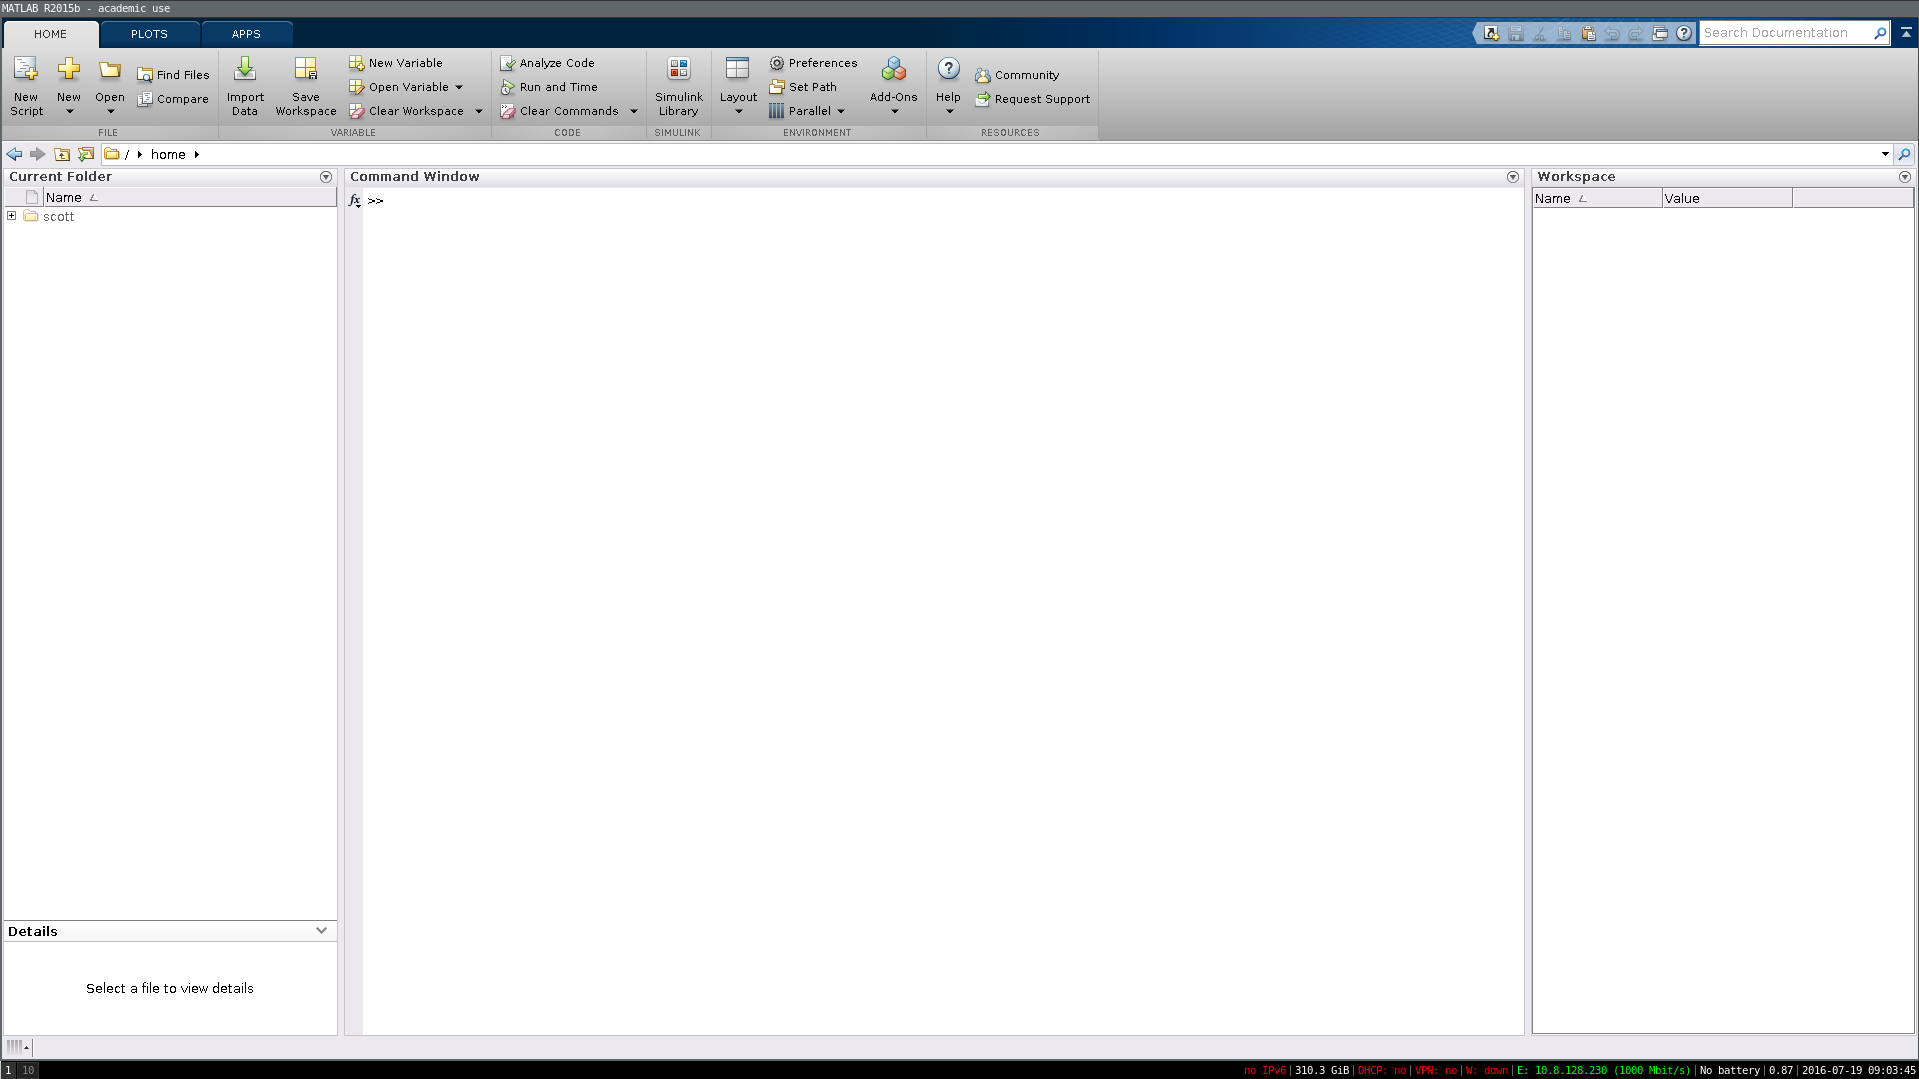
\includegraphics[width=1\textwidth]{matlab.png} 
    \caption*{}
\end{figure}
\item The main window in the centre is the \textit{command window} and contains the \textit{command prompt}. You can enter commands directly at the command prompt and Matlab will give some sort of output. The left hand side shows the current directory and the folder structure. This will be important later.
\item Calculations can be carried out in the usual way and follow the usual rules for ordering of operations. The figure below shows some example commands. After running these commands, you should note now that the \textit{workspace} on the right hand side contains a new value. This \textit{ans} variable takes the value of the last entered command - in this case, $5.75$.
\begin{figure}[h]		
	\centering
	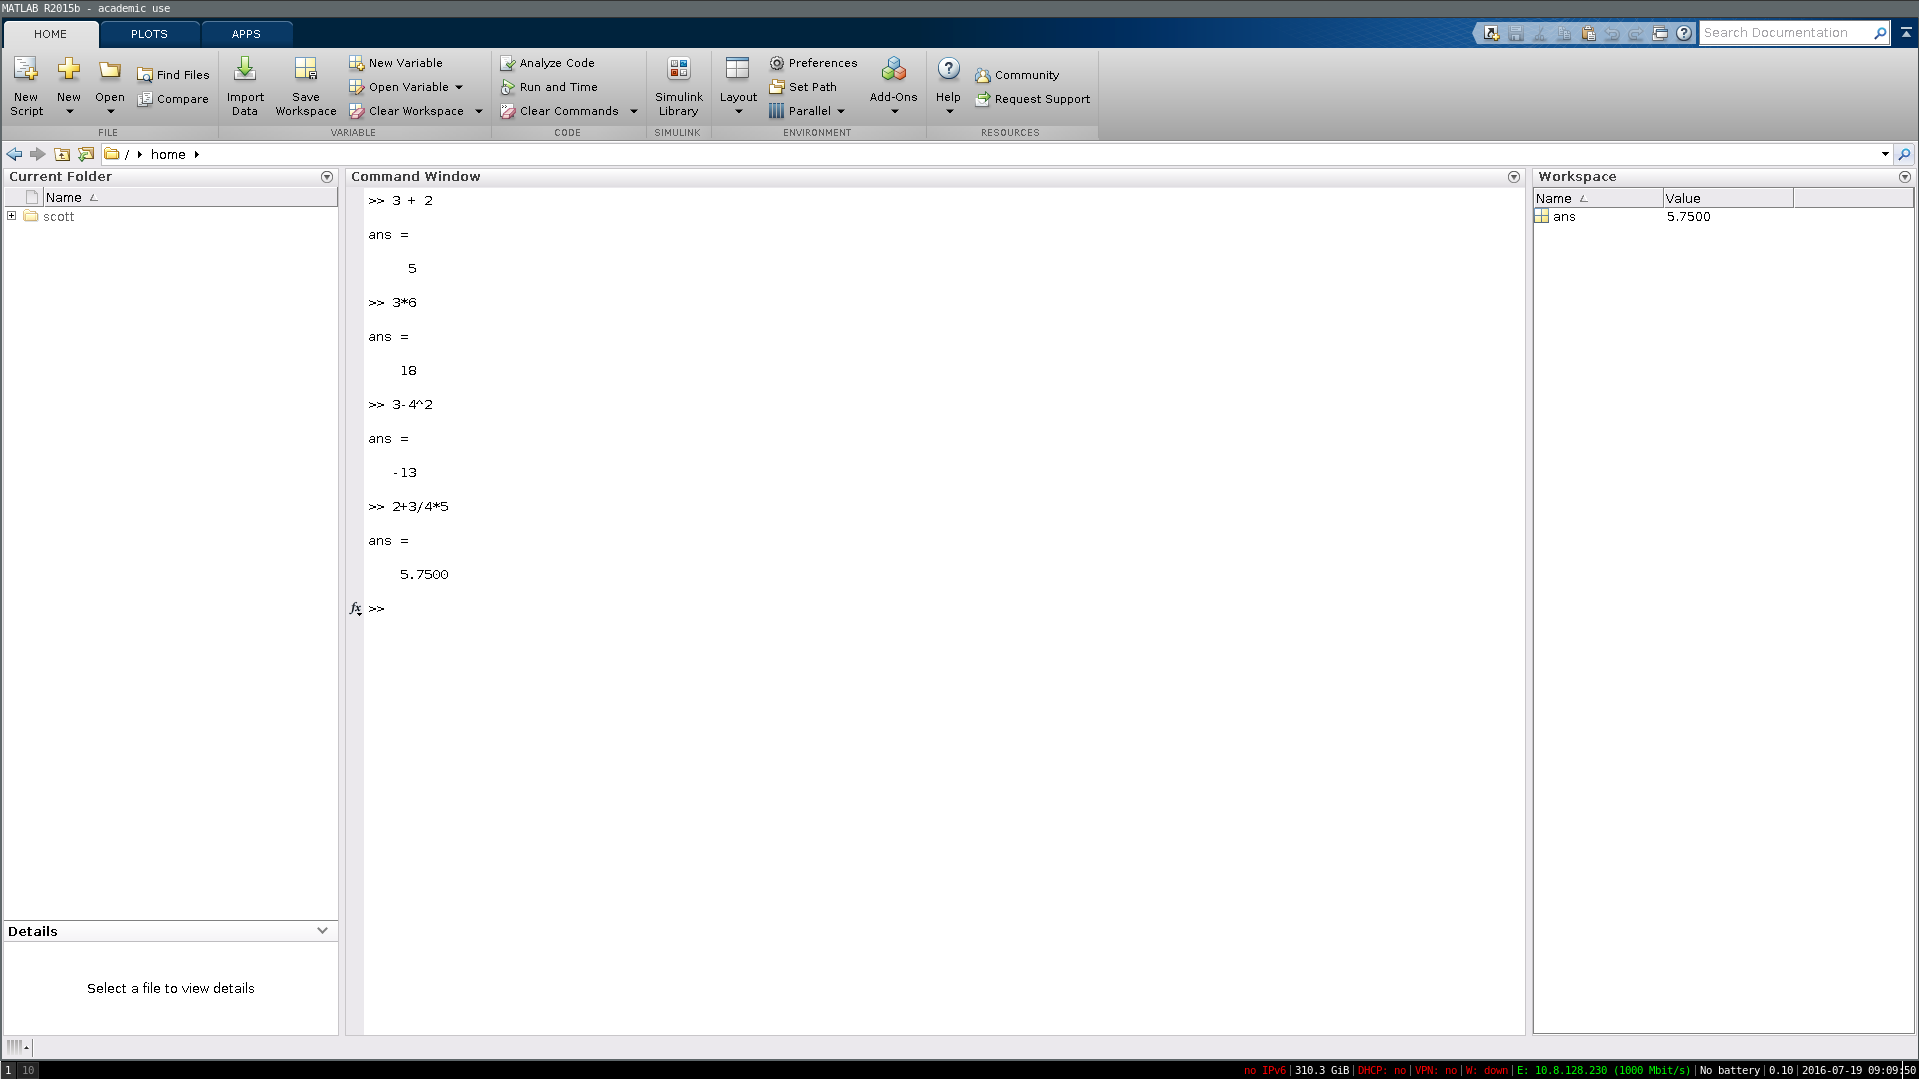
\includegraphics[width=1\textwidth]{matlabcalc.png} 
    \caption*{}
\end{figure}
\item While in theory you can work entirely in the command window, in practise this will get very untidy very quickly and so most of the calculations we will do will be inside what are called \textit{scripts}.
\item Scripts are basically text files which can be \textit{called} from inside the command window. Follow the procedure below to create a script.
\begin{itemize}
\item In the top left corner of the screen, click the yellow plus sign above the word \textit{new}.
\item Click script.
\item A window called \textit{Editor} should now appear above the command window, with the script named as \textit{untitled}.
\item To use the script, type a calculation into the Editor and save the file \textit{in the current directory} as \textit{test.m}
\item The script is then \textit{called} in the command window by writing 
\begin{lstlisting}
>> test
\end{lstlisting} 
at the prompt. The figure below shows the process.
\begin{figure}[h]		
	\centering
	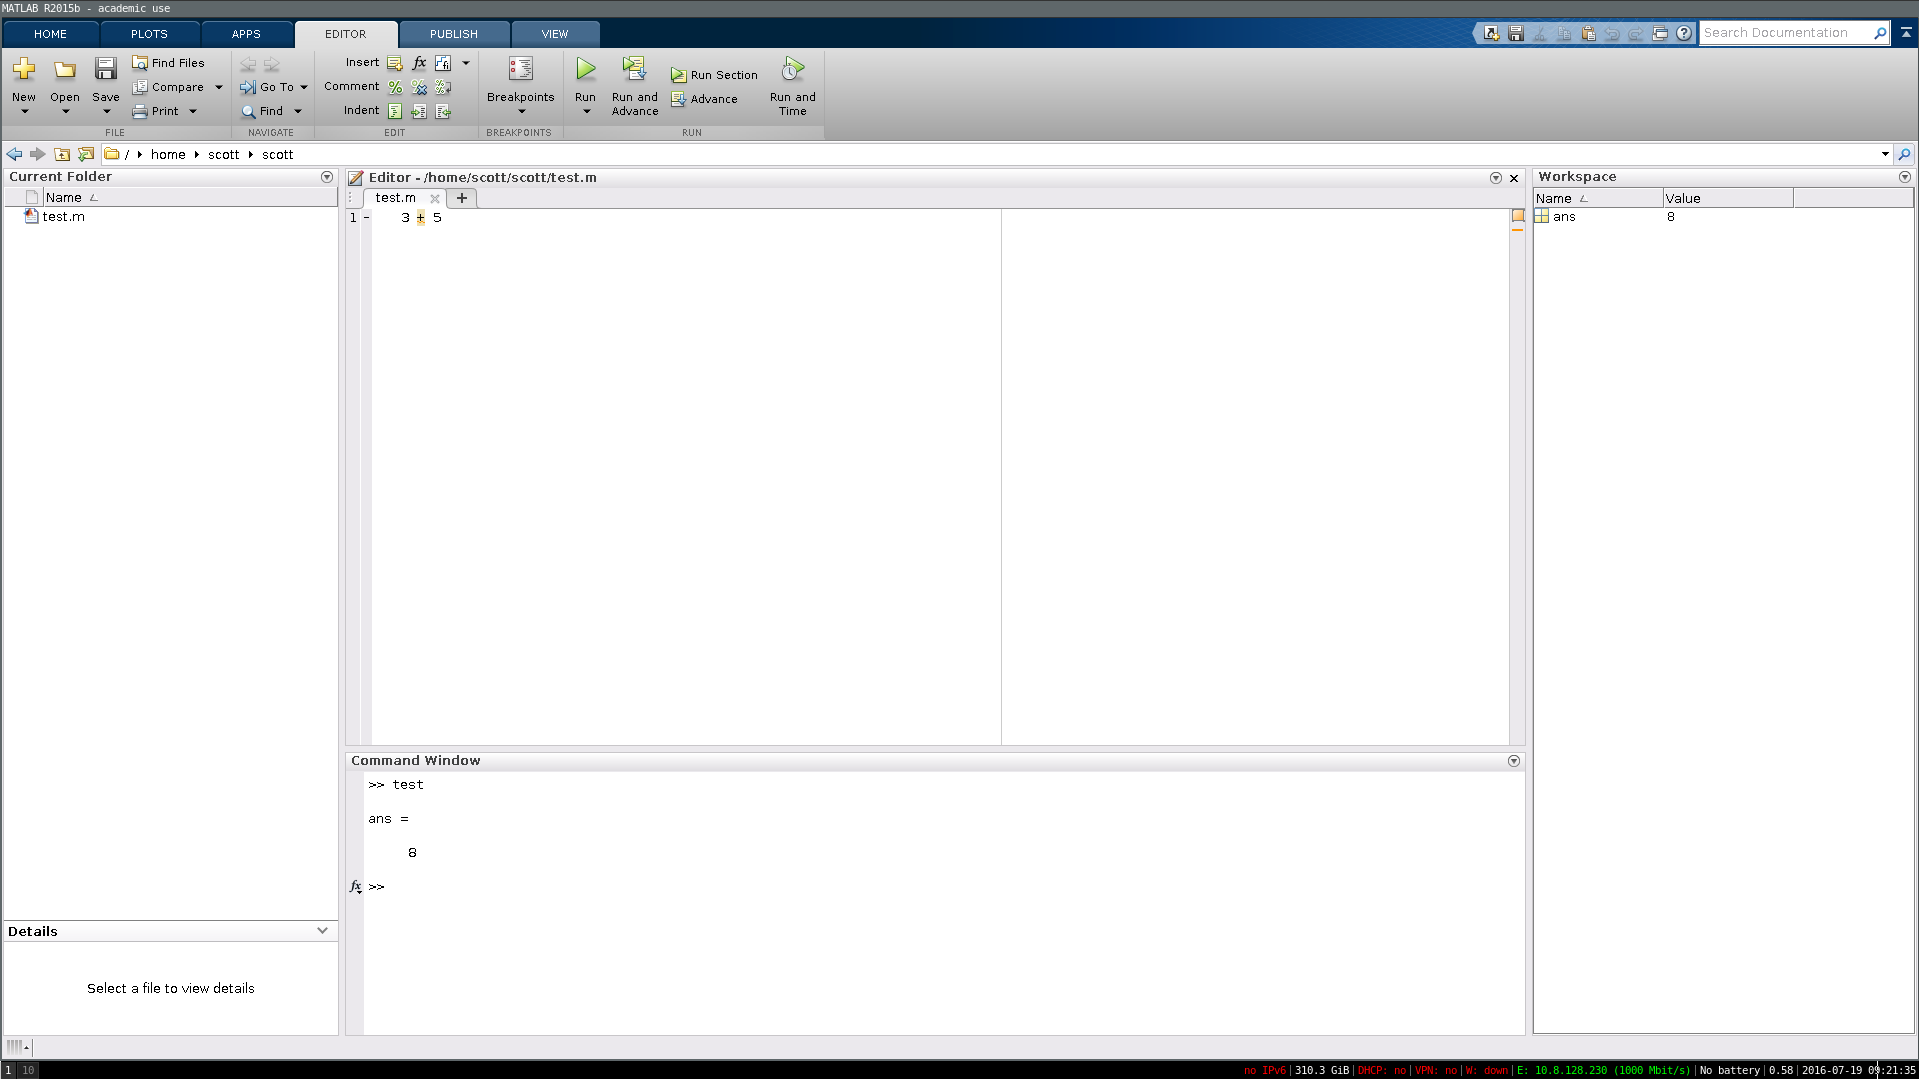
\includegraphics[width=1\textwidth]{matlabscript.png} 
    \caption*{}
\end{figure}
\end{itemize}
\item Now that you know the basic ideas behind creating a script and running commands in Matlab, you can start to have a play around with the interface. Matlab has lots of built in functions like \textit{sin, cos, tan, exp, log, abs, pi, sqrt} and many more. The best resource by far is Google! If you think Matlab may have a built in function that you want to use then chances are it does.
\item The command 
\begin{lstlisting}
>> demo
\end{lstlisting} 
is a great place to start learning about what everything does.
\end{itemize}

\subsection*{Remarks}

\begin{itemize}
\item Before we start getting into the basics of coding, there are a few remarks to make.
\begin{itemize}
\item There is more than one way to write a program! People have \textit{styles}, as you'll begin to see soon. If your program is different to mine then that's not a problem - you will develop your own way of doing things, your own way of naming things and as long as you're consistent with yourself then it won't matter. Someone once described it to me as learning a language, but with an accent - we can all understand each other but we say things in a slightly different way! It's like that with programming, don't be worried if your program looks different - if the results are the same it shouldn't matter too much.
\item \textit{However}, that being said, you should always strive to write code that is \textit{readable by another person}! You should always write comments explaining what complicated lines do and write your algorithms in a coherent way. This is not exclusive to your code being readable by someone else either - if you write a code that is not properly commented and don't look at it for a few months, you will not have any idea what it does the next time you look at it! This has happened to me so many times that I am determined to not let you make that mistake.
\end{itemize}
\item A \textit{comment} in Matlab is achieved with the \textit{\%} sign:
\begin{lstlisting}
>> 3 + 4; %this is a comment - it won't alter the result
\end{lstlisting} 
\item Using a semi-colon will \textit{suppress} the output of the command - and the answer will not be printed to the command prompt.
\end{itemize}

\section*{Basic Coding Ideas}

\subsection*{Variables}

\begin{itemize}
\item You can assign a value to a \textit{variable} in the following way
%
\begin{lstlisting}
>> x = 3; %assigns the value 3 to the variable x
\end{lstlisting}
%
This will give the variable \textit{x} the value 3, which can then be used in future calculations such as
%
\begin{lstlisting}
>> x = 3; %assigns the value 3 to the variable x
>> 3 + x %uses the assigned value in the calculation 3+x 
ans =
	6
\end{lstlisting}
%
These values will remain until they are overwritten or \textit{cleared}. You can clear specific variables using the \textit{clear} command.
%
\begin{lstlisting}
>> x = 3;
>> 3 + x
ans =
	6
>> clear x;
\end{lstlisting}
%
Trying to use the variable \textit{x} again will result in an error.

\item Unlike many other programming languages such as VB, Fortran or C++, there is no need to \textit{declare} variables to have a certain \textit{type} in Matlab. Matlab will automatically figure out whether you are specifying an integer, a real number or a complex number. 

\item Variables can be named any combination of letters and numbers both lower case and upper case but must start with a letter. 

\item You can see the variables which are currently stored by Matlab in the \textit{workspace}. Alternatively, you can see the same information by running the command
%
\begin{lstlisting}
>> whos
\end{lstlisting}
%
\end{itemize}

\subsection*{Loops}

If there is nothing else you take from this document, let the thing you learn be how to use \textit{for} loops and \textit{if} statements. These are central to most programs you will write during this course and usually play an important role in many other programs.

The very simple example below illustrates what these statements do.

\begin{lstlisting}
for j = 1:10
	disp(j) %display the value assigned to j at each point in the loop
end

for j = 1:10
	if j == 5
		disp(j + 3) %if j = 5, display the value 8 - i.e. 5+3
	elseif j == 6
		disp(j + 1) %if j = 6, display 7 - i.e. 6+1
	else
		disp(j) %if j is not equal to 5 or 6, display j
	end
end

\end{lstlisting}

\subsubsection{Remarks on Loops}

\begin{itemize}
\item You can use any variable you like as a loop counter name, although most people use $i$ or $j$. However, care must be taken when doing this. Matlab recognises $i$ and $j$ to mean complex $i$ unless they are user-defined first (i.e. at the start of a loop). Therefore, standard Matlab practise is to use $1i$ as complex $i$ and allow you to change the value of $i$ in a loop. If you want to input a complex number in Matlab, you should write it like this
\begin{lstlisting}
>>> 2 + 1i
\end{lstlisting}
\item Inside an if statement you can use several identities to check for conditions. The main ones are 
\begin{itemize}
\item $==$ (is equal to)
\item $\sim =$ (is not equal to)
\item $>=$, $>$ (is greater than or equal to, is greater than, similar for less than)
\item You can combine conditions with $\&\&$ (and) and $||$ (or).
\end{itemize}
\item There is another type of loop called a \textit{while} loop. These are similar to for loops but are particularly advantageous when you don't know how many iterations you need to end the loop. An example is below and one will need to be used in the tasks that follow.
\clearpage
\begin{lstlisting}
j = 1; %initialsise the variable j to have value 1 - why?
while j <= 10 %loop until j reaches 10
    disp(j) %output j at each step
    j = j + 1; %add one to j and loop again
end
\end{lstlisting}
\end{itemize}

\begin{tcolorbox}[title=Task]
  Write a script that will loop through the numbers 1 to $N$ and print out all numbers that are a multiple of 3. \newline
  \textit{Hint: You may find the following useful.}
  \begin{lstlisting}
  >> help mod
  \end{lstlisting}
  \tcblower
  \textit{Extension:} Extend the program so that it reproduces the game \textit{Fizzbuzz}. Have the code display the word \textit{Fizz} when it encounters a multiple of 3, \textit{Buzz} on a multiple of 5 and \textit{FizzBuzz} on a multiple of both 3 and 5.
\end{tcolorbox}

\begin{tcolorbox}[title=Task]
  Write a script that will check the Collatz\footnote{This is an open problem - no one has proved it for all $N\in\mathbb{N}$} conjecture for some number $N$.
  \tcblower
  \textit{The Collatz conjecture goes like this: 
  \begin{enumerate}
  \item Pick a number.
  \item If the number is even, halve it.
  \item If the number is odd, multiply it by $3$ and add $1$.
  \item Conjecture: the sequence will always reach $1$ in a finite number of steps.
  \end{enumerate}}
\end{tcolorbox}

\subsection*{Plotting}
\begin{itemize}
\item There are an overwhelming amount of possibilities that Matlab offers with regard to plotting functions - just describing it could be a course of its own. Therefore, in the interest of concision, I will only outline the absolute basic way of plotting here. You will pick up more points as you play around, but for now just see the following:
\begin{lstlisting}
  >> x = linspace(0,1,10); %generates grid of 10 points in [0,1]
  >> y = sin(x); %evaluates sin(x) at each of the 10 points 
  >> plot(x,y) %plots
\end{lstlisting}
\end{itemize}

\begin{tcolorbox}[title=Task - Quick]
  Plot the graph of $y = \cos(3x)$. Experiment with changing the value of the number of points plotted across. Plot the graph with circles at each point instead of a line using
  \begin{lstlisting}
    >> plot(x,y,'o')
  \end{lstlisting}
  To plot multiple things on the same figure, the command 
  \begin{lstlisting}
  >> hold on;
  \end{lstlisting}
  is useful, and can be used in the following way:
  \begin{lstlisting}
  >> plot(x,cos(x)); hold on;
  >> plot(x,sin(x))
  \end{lstlisting}
\end{tcolorbox}

\subsection*{Vectors \& Arrays}
\begin{itemize}
\item Matlab stores vectors in a very intuitive way and there are several ways to create them.
\begin{lstlisting}
>> u = [1 3 6]; %gives row vector containing 1, 3 and 6
>> v = 1:4; %gives row vector containing integers 1,2,3,4
>> w = 1:2:9; %gives row vector containing 1,3,5,7,9
>> for j = 1:4
		p(j) = j+1; %gives row vector containing 2,3,4,5
   end
\end{lstlisting}
\item The elements of the vector can be accessed by the notation $v(j)$, where $v$ is your variable name and $j$ is the number of the index you want to access. Note that Matlab indexing \textit{starts} at $1$. It is never possible to access $v(0)$.
\item Therefore, we can get the value $9$ from $w$ by typing 
\begin{lstlisting}
>> w(5)
ans = 9
\end{lstlisting}
\item Column vectors can be defined as transposes of row vectors or with the notation
\begin{lstlisting}
>> c = [1; 3; 5]; %note semi-colons. Row vectors are r = [1 3 5];
\end{lstlisting}
\item The transpose operation is 
\begin{lstlisting}
>> c' %this will trasnform a row into column and vice-versa
\end{lstlisting}
\end{itemize}

\begin{tcolorbox}[title=Task]
	Write a script that will print out the first $N$ Fibonacci numbers. An example code with bugs is available on the github page, under $\text{programs/mistakes/m3\_fib.m}$ Download this code and figure out what the problem is.
	\tcblower
	\textit{Extension:} Have a play around with the following command:
	\begin{lstlisting}
	%Display a header line. num2str changes with the value of N.
	disp(['The first ' num2str(N) ' terms are:']);
	\end{lstlisting}
	
	to format your output so that it's easily readable.
\end{tcolorbox}

\begin{tcolorbox}[title=Task]
  Use your previous Fibonacci program to plot the convergence of the ratio of successive terms to the golden ratio. \textit{Hint: Similarly to the loop in the previous exercise, set up a loop which stores the ratio terms $\frac{F_{n+1}}{F_{n}}$ in a vector $R$. Then compare this ratio to $\frac{1 + \sqrt{5}}{2}$.}
  \tcblower
  It can be shown that $\frac{F_{n+1}}{F_{n}} \to \frac{1 + \sqrt{5}}{2} =: \varphi$ as $n \to \infty$. You program should plot both the ratio calculated and the value $\varphi$ on the same axis.
\end{tcolorbox}

\begin{tcolorbox}[title=Task]
  Use your previous Collatz program to plot the route of the sequence to its final value $1$.
  \tcblower
  This will mean that you will have to store the values of $N$ in a vector as you go through the loop and then plot them.
\end{tcolorbox}

\begin{tcolorbox}[title=Task - Difficult]
  Write a script that will count and list the number of primes less than a given number $N$. This is called $\pi(N)$.
  \tcblower
  Extension: Compare your answer with the estimates $\pi(N) \approx N/log(N)$ and $\pi(N) \approx Li(N) := \int_0^N \frac{dt}{ln(t)}$. \textit{Hint: Matlab has a built in function for $Li$ called logint}. \textit{Hint: To check that a number $P$ is prime, you only need to check divisibility by numbers up to $\sqrt{P}$}
\end{tcolorbox}

\clearpage

\section*{Matlab Specific Coding Ideas}

\subsection*{Functions}

\begin{itemize}
\item Until now, everything you have written has been in the form of a \textit{script}. While that is useful, many programs will require the use of \textit{functions}.
\item A function contains parts of a code that need to be called in several places, to save you having to repeat code several times. The syntax and an example is below
\begin{lstlisting}
function c = myfunction(a,b) %function inputs a,b - outputs c
	c = a*b; %multiplies a and b - stores in c
end
\end{lstlisting}
\item The function is then called from the command prompt as
\begin{lstlisting}
>> c = myfunction(3,2)
c = 
	6
\end{lstlisting}
\item This function should be written in a script and saved with the \textit{same name as the function} in the current directory.
\end{itemize}

\begin{tcolorbox}[title=Task]
  Go back through your programs and change them into functions, with $N$ as an input wherever possible.
\end{tcolorbox}

\subsection*{Matrices}

\begin{itemize}
\item One of Matlab's huge advantages over its competitors is the way it handles operations with matrices. 
\item There are some immensely powerful tools that make many matrix calculations simple in Matlab that are very difficult to implement in some other programming languages. 
\item For example, Matlab has inbuilt commands for matrix multiplication, inversion, calculating eigenvalues, solving systems of equations, creating diagonal matrices, determinants and many many more. Before you go any further, think of what it would take to write a program for any of these things. Could you write a code that calculates the eigenvalues of any given matrix?
\item Matrices are formed in Matlab to a very similar way to vectors, and simply take two indices in an intuitive way
\begin{lstlisting}
for i = 1:N
	for j = 1:N
		A(i,j) = %some condition on the entries of A
	end
end
\end{lstlisting}
\item The elements of $A$ are then accessed similarly to vectors. For example, $A(1,3)$ will give you the entry in the 1st row and 3rd column of $A$.
\item Some standard commands are explained below. If there is a command which I've missed that you think should exist - chances are it probably does. Google is the answer!
\begin{lstlisting}
>> det(A); %determinant
>> inv(A); %inverse
>> A'; %transpose
>> A*B; %multiplication (note #columns of A = #rows of B)
>> A.*B; %Hadamard (entrywise) multiplication
>> ones(10); %creates a 10x10 matrix of ones
>> zeros(3,4); %creates a 3x4 matrix of zeros
>> diag(1:4); %a 4x4 diagonal matrix with 1 to 4 on the diagonal
>> eye(3); %the 3x3 identity matrix 
>> rand(3,2); %a 3x2 matrix of random numbers
\end{lstlisting}
\end{itemize}

\begin{tcolorbox}[title=Task - Quick]
	 Write a script that will create an $N \times N$ identity matrix using for loops and if statements. Check against eye(N).
\end{tcolorbox}

\begin{tcolorbox}[title=Task (Matrix Multiplication Algorithm)]
This is an exercise that will enable you to multiply two $N\times{N}$ matrices i.e. for a given matrix $A=a_{ij}$ and $B=b_{ij}$ write a code that computes $C=A\times{B}$
\vspace{5mm}

(i) Using either the \textit{randi} or the \textit{rand} function generate two $N\times{N}$ matrices $A$ and $B$  and initialize a third $N\times{N}$ matrix $C1$ using \textit{zeros}.
\vspace{2mm}

(ii) Write a \textit{for} loop to compute $A\times{B}$ \textbf{without} using MATLAB's matrix multiplication function.
 
\end{tcolorbox}

\subsection*{Systems of Linear Equations}

\begin{itemize}
\item Matlab has a particularly powerful tool for solving systems of equations called \textit{mldivide}, more commonly known simply as \textit{backslash}.
\item Given an matrix $A$ and a right hand side vector $b$, the solution vector $x$ which solves $Ax = b$ is calculated simply by
\begin{lstlisting}
>> A = rand(10); b = rand(10,1);
>> x = A\b;
\end{lstlisting}
\item Of course for this example the following would be equivalent
\begin{lstlisting}
>> A = rand(10); b = rand(10,1);
>> x = inv(A)*b;
\end{lstlisting}
but this is considered bad practise as there is no need to calculate the inverse to solve the problem - leading to an increase in computational time. If you try to solve the problem in this way, Matlab will shout a warning.
\item Backslash can also be used to solve over- and under- determined systems of equations in a similar way and uses least-squares fitting to do so. It is a very powerful tool which has made Matlab very popular for matrix operations.
\item The command
\begin{lstlisting}
>> help mldivide
\end{lstlisting}
will give a good explanation of the methods used and the best practice usage of this operator.
\begin{tcolorbox}[title=Task]
	Solve the system of equations 
	\begin{align*}
	3x + 4y + 7z &= 32 \\
	x + 5y + 2z &= 17 \\
	2x + y + z &= 7
	\end{align*}
	and compare the time taken between backslash and inverse multiplication.
	\tcblower
	\begin{itemize}
	\item To create the matrix above in Matlab, you can use the vector-type notation discussed above. In particular, the command
	\begin{lstlisting}
	>> A = [3 4 7; 1 5 2; 2 1 1];
	\end{lstlisting}
	will create the matrix on the left hand side, while
	\begin{lstlisting}
	>> b = [32; 17; 7];
	\end{lstlisting}
	will create the right hand side.
	\item 	To measure the time taken by a script (in this case called \textit{test.m}), use the following
	\begin{lstlisting}
	>> tic, test; toc
	\end{lstlisting}
	\end{itemize}
\end{tcolorbox}
\item Hopefully the following example will convince you to use backslash! 
\begin{lstlisting}
>> A = diag(rand(5000,1)); b = rand(5000,1);
>> tic, x = inv(A)*b; toc
Elapsed time is 30.292078 seconds.
>> tic, x = A\b; toc
Elapsed time is 0.040788 seconds.
\end{lstlisting}
\end{itemize}

\subsection*{Eigenvalues \& Eigenvectors}

\begin{itemize}
	\item Another important feature of Matlab's matrix capabilities is its ability to calculate eigenvalues and eigenvectors of matrices.
	\item Given a matrix $A$, the eigenvalues and eigenvectors can be calculated simply using
	\begin{lstlisting}
	>> [V,D] = eig(A);
	\end{lstlisting}
	\item This effectively solves the problem
	\begin{displaymath}
	Av = \lambda v
	\end{displaymath}
	and stores the vectors $v$ in $V$ and the corresponding eigenvalues $\lambda$ along the diagonals of the diagonal matrix $D$.
	\item Time-permitting, we may revisit this later in the course, but for now it is useful to just know that it exists.
\end{itemize}


\section*{Some More Advanced Ideas - with Applications in Applied Mathematics}

\begin{itemize}
	\item The following section will be organised into four/five distinct parts. We may not have time to cover them all, but they will be included for reference anyway.
	\begin{enumerate}
		\item Numerical integration via the trapezium rule.
		\item Solving linear ODEs with inbuilt functions.
		\item Newton's method for root-finding.
		\item Simple finite difference solutions to ODEs.
		\item A brief introduction to spectral methods.
	\end{enumerate}
	\item Note that this course is NOT intended to be about the mathematical justification of the methods involved. We will likely be sloppy with assumptions and not get too heavily involved in the analysis. Take me at my word for now that these methods are valid - the MAGIC course on Numerical Analysis as well as the MMath course on fluid dynamics will reinforce the ideas presented here if the interested student would like to know more.
\end{itemize}

\subsection*{Numerical Integration}

\begin{itemize}
	\item Matlab has a useful inbuilt function for calculating integrals via the trapezium rule called \textit{trapz}. Example usage can be found via
	\begin{lstlisting}
	>> help trapz
	\end{lstlisting}
	\begin{tcolorbox}[title=Task]
		Write a function which will integrate some input function $y$ over a user-defined interval $[a,b]$. Your function should compare the results with the exact answer and make it simple to alter the function being integrated if required. 
		\tcblower
		Experiment with the accuracy obtained by altering the number of grid points taken.
	\end{tcolorbox}
\end{itemize}

\subsection*{Solving linear ODEs}

\begin{itemize}
\item To solve an ODE numerically, we can use Matlab's built in tools called \textit{ode23} and \textit{ode45}. These can be used to solve equations of the form 
\begin{displaymath}
\frac{dy}{dt} = f(t); \hspace{3mm} y(y_0) = t_0
\end{displaymath}
or even higher order linear ODEs and systems of ODES. Typing
\begin{lstlisting}
>> help ode45
\end{lstlisting}
will give you plenty of information about the implementation of this routine, but I have included a full working example below to illustrate the usage. The code below solves the equation 
\begin{displaymath}
\frac{dy}{dt} = \cos(t); \hspace{3mm} y(0) = 2
\end{displaymath}
on the interval $[0, 2\pi]$.
\begin{lstlisting}
%Initialise solution parameters
a = 0; b = 2*pi; %Interval end points
y0 = 2; %Initial condition

[t23,y23] = ode23(@func,[a b],y0); %Solve using ode23

function f = func(t,y)
    f = cos(t); %right hand side.
end
\end{lstlisting}

\begin{tcolorbox}[title=Task]
Implement the routine above and also include the solution from \textit{ode45}. Compare the solutions to the exact solution $y = 2 + \sin(t)$. What do you notice? Which is more accurate?
\end{tcolorbox}

\item You can also use \textit{ode23/45} to solve second or higher order linear ODEs if you reformulate them as linear systems of ODEs first. Assume we have
\begin{align*}
y'' + \exp(t)y' + ty(t) = 3\sin(2t) \\
y(0) = 2; \hspace{3mm} y'(0) = 8
\end{align*}
in the interval $[0, 4]$. Then we can let $x_1 = y$ and $x_2 = y'$ and write this as 
\begin{align*}
x_1' &= x_2 \\
x_2' &=  -tx_1 - \exp(t)x_1 + 3\sin(2t) \\
x_1&(0) = 2; \hspace{3mm} x_2(0) = 8
\end{align*}
\item We can then solve this system in a similar way to the first order case except now we will get a \textit{vector} of solutions. A full working script is below
\begin{lstlisting}
function ode

%Initialise solution parameters
a = 0; b = 4; %Interval end points
x0 = 2; x1 = 8; %Initial conditions

[t23,x23] = ode23(@func,[a b],[x0,x1]); %Solve using ode23

%Plots
plot(t23,x23(:,1),'b');
xlabel('t'); ylabel('y(t)'); xlim([min(t23) max(t23)]);

end

function f = func(t,x)
    f = zeros(2,1); % since output must be a column vector
    f(1) = x(2); 
    f(2) = -t*x(1)-exp(t)*x(2)+3*sin(2*t);
end
\end{lstlisting}
\item Note that the solution $y$ is stored in $x(:,1)$, while $y'$ would be stored in $x(:,2)$.
\begin{tcolorbox}[title=Task]
Implement the routine above for \textit{ode45}. Plot both solutions on the same axis and compare.
\end{tcolorbox}
\end{itemize}

\subsection*{Newton's method}

\begin{itemize}
\item Given an equation $f(x) = 0$, where $f$ is differentiable, we can iterate towards the root $x_r$ by means of Newton's method in the following way
\begin{displaymath}
x_{n+1} = x_n - \frac{f(x_n)}{f'(x_n)}
\end{displaymath} 
for some initial guess $x_0$. Provided we have a good initial guess, this will produce approximate solutions to any degree of accuracy required. In some cases, Newton's method requires the guess $x_0$ to be \textit{fairly close} to the true solution - something which is not always easy to do.
\begin{tcolorbox}[title=Task]
		Write a code that implements Newton's method for $f(x) = 0$ in the following cases:
		\begin{itemize}
		\item $f(x) = x^2 - 5$ with starting guess $x_0 = 2$.
		\item $f(x) = \sin(x)+x\cos(x)$ with starting guess $x_0 = 1.5$. Try the same function with $x_0 = 1$. What do you notice? Is this valid?
		\end{itemize}
		\tcblower
		Your code should be independent of your choice of function. Try to write the Newton method as its own function, and call your input functions separately. You should produce a table of the error in successive iterations and a plot of the convergence. In the first case, plot also the exact solution $x_r = \sqrt{5}$ and check your results. You can assume you have convergence when $|x_{n+1} - x_n| < 10^{-8}$
	\end{tcolorbox}
\end{itemize}

\subsection*{Finite Differences}

\begin{itemize}
\item Finite difference methods are a class of solution methods used widely in applications to solve complicated systems of ODEs.
\item By the process of discretising an ODE, we essentially replace the problem of finding
the exact, continuous solution with the problem of finding the values of
the solution at specified discrete points in space and time by deriving and solving an
appropriate set of algebraic equations. This discrete problem is only an approximation
to the problem, which improves as we increase the number of points we use.
\item A crucial step in the finite difference method (FDM) is the approximation of derivatives by finite differences (FD), i.e. the replacement of derivatives by some algebraic
formula.
\item The method relies on Taylor series expansions and I won't go into too much detail here. However, it does not take much thought to arrive at the following approximation for the derivative of a function $F$.
\begin{displaymath}
F'(x_n) \approx \frac{F(x_{n+1}) - F(x_n)}{x_{n+1}-x_n}
\end{displaymath}
which is basically just the GCSE formula $m = \frac{\Delta y}{\Delta x}$. This is called the \textit{forward-difference formula} and is \textit{first-order accurate}. This means that if we increase the resolution by $\frac{1}{10}$ then the accuracy of the solution also increases by $\frac{1}{10}$. This is not considered very accurate, and as such is rarely used.
\item The expression can be similarly derived by Taylor series expansions around $x_n$ and it is not much of a stretch to imagine a formula in the opposite direction, namely 
\begin{displaymath}
F'(x_n) \approx \frac{F(x_{n}) - F(x_{n-1})}{x_{n}-x_{n-1}}
\end{displaymath}
This is called the \textit{backward-difference formula} and is also first-order accurate. These two can be combined into a single, second-order accurate formula 
\begin{displaymath}
F'(x_n) \approx \frac{F(x_{n+1}) - F(x_{n-1})}{2h}
\end{displaymath}
where $h := x_{n}-x_{n-1}$. This is called the \textit{central difference formula}.
\item Similar formulae exist for higher order derivatives which we won't derive, but we state the second-order accurate central difference approximation to the second derivative as 
\begin{displaymath}
F''(x_n) \approx \frac{F(x_{n+1}) - 2F(x_n)  + F(x_{n-1})}{h^2}
\end{displaymath}

\end{itemize}

\subsubsection{An example with Matlab implementation}

\begin{itemize}
\item Suppose that we want to solve the boundary value problem 
\begin{displaymath}
u'' = f(x), \hspace{3mm} x \in (0,1)
\end{displaymath}
where we set
\begin{align*}
f(x) &= \pi^2\sin(\pi x) \\
u(0) &= 0; \hspace{3mm} u(1) = 1
\end{align*}
This has exact solution $u_e = x - \sin(\pi x)$ which we will use later to compare results.
\item We set up the grid in the $x$ direction in the usual way 
\begin{lstlisting}
N = 10; 
x = linspace(0,1,N+1); %N+1 domain points (gives spacing h = 1/N)
h = x(2)-x(1); %gives nodal spacing
\end{lstlisting}
\item At each \textit{interior} point $x_j$, $(j = 1,\ldots,N-1)$ in the domain, we can approximate the derivative $u''$ using our central difference formula as follows
\begin{displaymath}
\frac{U_{i+1} - 2U_i + U_{i-1}}{h^2} = f(x_i) \implies U_{i+1} - 2U_i + U_{i-1} = h^2f(x_i)
\end{displaymath}
Thus we can write the resulting algebraic system as (convince yourself this is correct!)
\begin{displaymath}
\left(\begin{matrix}
  1 & -2 & 1 & 0 & 0 & \ldots & 0 & 0 & 0 \\
  0 & 1 & -2 & 1 & 0 & \ldots & 0 & 0 & 0 \\
  0 & 0 & 1 & -2 & 1 & \ldots & 0 & 0 & 0 \\
  \vdots & \vdots & \vdots &  &  & & \vdots & \vdots & \vdots \\
  0 & 0 & 0 & \ldots & 1 & -2 & 1 & 0 & 0 \\
  0 & 0 & 0 & \ldots & 0 & 1 & -2 & 1 & 0 \\
  0 & 0 & 0 & \ldots & 0 & 0 & 1 & -2 & 1 \\
 \end{matrix}\right)
 \left(\begin{matrix}
 U_0 \\
 U_1 \\
 U_2 \\
 U_3 \\
 \vdots \\
 U_{N-3} \\
 U_{N-2} \\
 U_{N-1} \\
 U_N \\
 \end{matrix}\right)
 = h^2\left(\begin{matrix}
  f_1 \\
  f_2 \\
  f_3 \\
  \vdots \\
  f_{N-3} \\
  f_{N-2} \\
  f_{N-1} \\
  \end{matrix}\right)
\end{displaymath}
\item However, we already know the solutions at nodes $U_0 = u(0) = 0$ and $U_N = u(1) = 1$ so the first and last columns may be transferred to the right hand side to give
\begin{displaymath}
\left(\begin{matrix}
-2 & 1 & 0 & 0 & \ldots & 0 & 0 \\
1 & -2 & 1 & 0 & \ldots & 0 & 0 \\
0 & 1 & -2 & 1 & \ldots & 0 & 0 \\
\vdots & \vdots &  &  &  & \vdots & \vdots \\
0 & 0 & \ldots & 1 & -2 & 1 & 0 \\
0 & 0 & \ldots & 0 & 1 & -2 & 1 \\
0 & 0 & \ldots & 0 & 0 & 1 & -2 \\
\end{matrix}\right)
\left(\begin{matrix}
U_1 \\
U_2 \\
U_3 \\
\vdots \\
U_{N-3} \\
U_{N-2} \\
U_{N-1} \\
\end{matrix}\right)
= h^2\left(\begin{matrix}
f_1 \\
f_2 \\
f_3 \\
\vdots \\
f_{N-3} \\
f_{N-2} \\
f_{N-1} \\
\end{matrix}\right) - 
u(0)\left(\begin{matrix}
1 \\
0 \\
0 \\
\vdots \\
0 \\
0 \\
0 \\
\end{matrix}\right) - 
u(1)\left(\begin{matrix}
0 \\
0 \\
0 \\
\vdots \\
0 \\
0 \\
1 \\
\end{matrix}\right)
\end{displaymath}
\item By doing so, we isolate the unknown nodal values $U_i$, for $i = 1,\ldots,N−1$, on the left hand side, casting the global system of equations in the form $Au = g$.
\item To convert this into a MATLAB script, the main difficulty is in the construction of the matrix A. To do this we will use the \textit{diag} command which we introduced earlier. You could also do it with for loops, although there is no need here.
\begin{lstlisting}
% A diagonal matrix with -2 on the diagonal
D0 = -2*diag(ones(N-1,1));

% A matrix with 1 along the 1st superdiagonal
D1 = diag(ones(N-2,1),1); %

% A matrix with 1 along the 1st subdiagonal
D2 = diag(ones(N-2,1),-1);

% Construct the full matrix
A = D0 + D1 + D2;

% The right hand side of the BVP (x(2:N) gives interior nodes)
f = pi^2*sin(pi*x(2:N));

% The right hand side of the linear system
g = h^2*f;
g(1) = g(1) - 0; %not necessary, but illustrative
g(N-1) = g(N-1) - 1; %from boundary conditions
g = g'; %transpose for backslash solver
\end{lstlisting}
\clearpage
\item Finally we are left to solve and plot the solution
\begin{lstlisting}
u(1) = 0; u(N+1) = 1; %sets boundary conditions 
u(2:N) = A\g; %solves the system Au = g
plot(x,u)
\end{lstlisting}

\begin{tcolorbox}[title=Task]
Implement the above code in Matlab. Plot the result against the exact solution and quantify the error. Experiment with altering the value of $N$. Plot both exact solution and approximate solution on the same axes - use circles to denote the points at which the finite difference approximation is taken.
\end{tcolorbox}

\begin{tcolorbox}[title=Task]
Use finite difference methods to solve the \textit{convection-diffusion equation}
\begin{displaymath}
-\epsilon u''(x) + \beta u'(x) = 0; \hspace{3mm} u(0) = 1, \hspace{3mm} u(1) = 0
\end{displaymath}
and compare against the exact solution $u(x) = \left(\frac{\exp\left(\frac{\beta}{\epsilon}\right)-\exp\left(\frac{\beta}{\epsilon}\right)}{\exp\left(\frac{\beta}{\epsilon}\right)-1}\right)x$
\tcblower
Experiment with changing the values of $\epsilon$ and $\beta$. Start with $N=10$ and $\epsilon = 0.1$, $\beta = 0.5$. Then try $\epsilon = 0.01$, $\beta = 0.5$. What do you notice? Can you work out when \& why this happens? \textit{Hint: The ratio $\frac{\beta h}{\epsilon}$ is important}.
\end{tcolorbox}

\end{itemize}

\clearpage 

\section*{The Finite Element Method}

\newtheorem{theorem}{Definition}[section]
\newtheorem{proposition}{Proposition}[section]

\section*{Overview}
\begin{itemize}
\item The Finite Element Method (FEM) is another numerical method that is used to approximate solutions to boundary value problems (ODEs/PDEs).
\item Similar to Finite Differences, the Finite Element method solves boundary value problems by converting differential equations into systems of linear equations.
\item The solution of the linear systems provide a discrete set of points that the approximate the values of the function at those points.
\item FEM is extensively used in industrial modelling and engineering and is one of the most well known numerical methods for solving differential equations.
\item The spatial discretisation permitted by Finite Element modelling is especially useful when solving (2D) problems in irregular shaped domains that are cannot be discretized easily by finite differences.
\end{itemize}




\tikzstyle{startstop} = [rectangle, rounded corners, minimum width=3cm, minimum height=1cm,text centered, draw=black, fill=red!30]
\tikzstyle{io} = [trapezium, trapezium left angle=70, trapezium right angle=110, minimum width=3cm, minimum height=1cm, text centered, draw=black, fill=blue!30]

\tikzstyle{process} = [rectangle, minimum width=3cm, minimum height=1cm, text centered, draw=black, fill=orange!30]
\tikzstyle{decision} = [diamond, minimum width=3cm, minimum height=1cm, text centered, draw=black, fill=green!30]

\tikzstyle{arrow} = [thick,->,>=stealth] % Arrow Type

 

\begin{center}
\clearpage
\textbf{Finite Elemnt Method Implementation}
\vspace{5mm}

\begin{tikzpicture}[node distance=2cm]

\node (start) [startstop] {ODE/PDE};

\node (in1) [startstop, below of=start] {Weak Formulation};

\node (in2) [startstop, below of=in1] {Galerkin Approximation (Spatial Discretisation)};

\node (in3) [startstop, below of=in2] {Linear System};

\draw [arrow] (start) -- (in1);
\draw [arrow] (in1) -- (in2);
\draw [arrow] (in2) -- (in3);


\end{tikzpicture}

\end{center}

The Finite Element method can be broken down into 4 discrete stages:

\begin{itemize}
\item \textbf{ODE/PDE} - Formulation of the Boundary Value Problem needing to be solved.
\item \textbf{Weak Formulation} - Re-writing the problem in terms of \textit{inner products} using \textit{test functions}.
\item \textbf{Galerkin Approximation} - Restricting the weak problem to \textit{piecewise linear} functions.
\item \textbf{Linear System} - Constructing the Linear system of equations that represents the Galerkin (linear) approximation.
\end{itemize}

Note: Finite Element Analysis is difficult and requires extensive knowledge of functional analysis and linear algebra. In the context of this course we will avoid going into detail about some of the more technical aspects. If you want to find out more about FEA please let us know.

\section*{An Example of 1D FEM implementation}

Consider the same problem as discussed in the section on finite differences.
%
\begin{subequations}\label{BVP}
\begin{align}
u''(x)&=f(x)\qquad\textnormal{for}\qquad{-1}<x<1 \\
u(-1)&=1=u(1) \qquad f(x)=\pi^2\sin(\pi{x})
\end{align}
\end{subequations}
%
It is easy to verify that the solution to the BVP \eqref{BVP} is given by $$u(x)=1-\sin(\pi{x})$$. 

\subsection*{Weak Formulation}

\begin{itemize}
\item The weak formulation of a BVP is an alternate way of writing our problem using \textit{bilinear forms}.
\item It requires the use of \textit{test functions} that belong to certain function spaces.
\item The weak form of the differential equation given by \eqref{BVP} requires the following function spaces.
\end{itemize}

\begin{equation}\label{Vspace}
V=\Bigg\{v(x):\quad\int_{-1}^{+1}|v(x)|^2+|v'(x)|^2\,dx<\infty, \quad v(\pm{1})=0\Bigg\}
\end{equation}


\begin{equation}\label{Wspace}
W=\Bigg\{w(x):\quad\int_{-1}^{+1}|w(x)|^2\,dx<\infty, \quad w(\pm{1})=0\Bigg\}
\end{equation}


First multiply \eqref{BVP} by a test function $v\in{V}$ and integrate over $[-1,1]$

\begin{equation}\label{BVPtest}
\int_{-1}^{+1}u''(x)v(x)\,dx=\int_{-1}^{+1}f(x)v(x)\,dx
\end{equation}

Using \textit{integration by parts} the LHS

\begin{equation}\label{BVPparts}
[u(x)v(x)]^1_{-1}-\int_{-1}^{+1}u'(x)v'(x)\,dx=\int_{-1}^{+1}f(x)v(x)\,dx
\end{equation}

Using the fact that $v(\pm{1})=0$  

\begin{equation}\label{BVPweak}
\int_{-1}^{+1}u'(x)v'(x)\,dx=-\int_{-1}^{+1}f(x)v(x)\,dx
\end{equation}

Eq. \eqref{BVPweak} is known as the \textit{weak form} of \eqref{BVP}. Using inner product notation $\int_{\Omega}fg\,d\Omega=(f,g)$

\begin{equation}
(u',v')=-(f,v)
\end{equation}

The weak form of the equations is then: Find $u\in{W}$ such that 

\begin{equation}\label{BVPweaklin}
a(u,v)=-l(v)\qquad\forall{v\in{V}}
\end{equation}

where $a(u,v)=\int_{-1}^{+1}u'(x)v'(x)\,dx$ and $l(v)=\int_{-1}^{+1}f(x)v(x)\,dx$.


\subsection*{Galerkin Approximation}
\begin{itemize}
\item The objective now is to find \textit{piecewise linear} functions that approximate the solution to \eqref{BVPweaklin}.
\item  The trial space, V, and test space, W, in the weak formulation
are replaced by subspaces comprising polynomials of degree $1$. These subspaces are denoted by $V^h$ and $W^h$ respectively, i.e. $V^h⊂V$ and $W^h⊂W$.
\item As with the case for finite differences divide the interval $[−1, 1]$ into $N$ subintervals (elements) $[x_{k−1} , x_k]$, $k = 1, . . . , N$ with $x_0=−1$ and $x_N = 1$.
\end{itemize}

Consider a piecewise linear approximation to $u(x)$ and $f(x)$ given by

\begin{equation}\label{linappu}
u(x)\approx{u}^h(x)=U_0\phi_0(x)+...+U_N\phi_N(x)
\end{equation}

\begin{equation}\label{linappf}
f(x)\approx{f}_0\phi_0(x)+...+f_N\phi_N(x)
\end{equation}

where $\phi_i(x)$ are piecewise linear basis functions (hat functions).

\begin{itemize}
\item As in the case of finite differences, the goal is to construct a (linear) system of
equations to solve for the unknown nodal values of $u^h$: $U_i$ ($i=1,..,N-1$)
\end{itemize}

\subsubsection*{Basis Functions}

In the kth element there are two local basis functions

\begin{equation*}
\psi_{1,k}=\frac{x_{k}-x_{k-1}}{h}\qquad\psi_{2,k}=\frac{x_{k+1}-x_{k}}{h}
\end{equation*}

The basis functions $\phi_j(x)$ are then defined 

\[\phi_{j}(x)= \begin{cases} 
      \psi_{j,2}(x) & x_{j-1}\leq x\leq x_j  \\
      \psi_{j+1,1}(x) & x_{j}\leq x\leq x_{j+1} 
   \end{cases}
\]

for interior nodes $j=1,2,..N-1$ and at the boundary nodes $x_0$ and $x_{N}$ 

\[\phi_{1}(x)= \begin{cases} 
      \psi_{1,1}(x) & x_0\leq x\leq x_1 \\
       0 &  \quad\textnormal{otherwise} 
   \end{cases}
\]

\[\phi_{N}(x)= \begin{cases} 
     \psi_{2,N}(x) & x_{N-1}\leq x\leq x_{N} \\
       0 &  \quad\textnormal{otherwise} 
   \end{cases}
\]

\begin{figure}[h!]\label{hatfunc}
\begin{center}
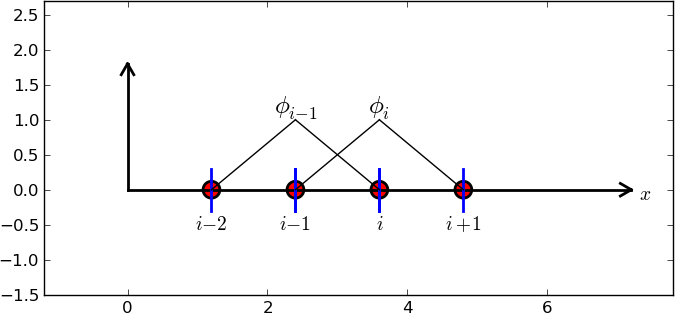
\includegraphics[width=60mm]{hatfunction.png}
\caption{The basis function $\phi_k$ at $k=i-1$ and $k=i$. The basis functions are such that $\phi_i(x_i)=1$ and $\phi_i(x_j)=0$ $j\neq{i}$}
\end{center}
\end{figure}

\begin{itemize}
\item Substituting the approximations \eqref{linappu} and \eqref{linappf} into \eqref{BVPweaklin} we get the following 
\end{itemize}

\begin{equation}\label{BVPgaler}
a(u^h,v^h)=-l(v^h)
\end{equation}

\begin{equation}
a\Bigg(\sum^{N}_{j=0}{U}_{j}\phi_j(x),\phi_i(x)\Bigg)=-\Bigg(\sum^{N}_{j=0}f_j\phi_j(x),\phi_i(x)\Bigg)
\end{equation}

\begin{equation}\label{BVPgaler}
\sum^{N}_{j=0}{U}_{j}a\Bigg(\phi_j(x),\phi_i(x)\Bigg)=-\sum^{N}_{j=0}f_j\Bigg(\phi_j(x),\phi_i(x)\Bigg)
\end{equation}

\begin{equation}\label{BVPgalersys}
\sum^{N}_{j=0}{U}_{j}A_{ij}=-\sum^{N}_{j=0}M_{ij}f_j
\end{equation}


\subsection*{Matrix Assembly}

Equation \eqref{BVPgalersys} represents a \textit{linear system of equations} of the form $A\textbf{u}=-M\textbf{f}$. We now have to construct the matrices $A$ and $M$ in order to 


\subsubsection{Local Matrix Construction}

\begin{itemize}
\item In this 1D example, this means that we have to only consider the interactions of the
two element basis functions that are local to the kth element, $\psi_{1,k}(x)$ and $\psi_{2,k}(x)$.
\item For a 1D problem the stiffness matrix local to the kth element is the ${2}\times{2}$ matrix defined in terms of the local basis functions by
\end{itemize}

\begin{equation}
A^{(k)}_{\alpha,\beta}=\int_{x_{k-1}}^{x_{k}}\psi'_{\alpha,k}\psi'_{k,\beta}\,{dx}=\frac{(-1)^{\alpha+\beta}}{h}\qquad{\alpha,\beta=1,2}
\end{equation}

Similarly the local mass matrix is given by 

\begin{equation}
M^{(k)}_{\alpha,\beta}=\int_{x_{k-1}}^{x_{k}}\psi_{\alpha,k}\psi_{k,\beta}\,{dx}\qquad{\alpha,\beta=1,2}
\end{equation}

\begin{equation}
\begin{split}
M^{(k)}_{1,1}&=\frac{1}{h^2}\int_{x_{k-1}}^{x_{k}}(x_k-x)^2\,{dx}=\frac{h}{3}\qquad{M}^{(k)}_{2,2}=\frac{1}{h^2}\int_{x_{k-1}}^{x_{k}}(x-x_{k-1})^2\,{dx}=\frac{h}{3}\\
&{M}^{(k)}_{1,2}={M}^{(k)}_{2,1}=\frac{1}{h^2}\int_{x_{k-1}}^{x_{k}}(x_k-x)(x-x_{k-1})\,{dx}=\frac{h}{6}
\end{split}
\end{equation}


Thus the 

\[A^{(k)} = \frac{1}{h}
 \begin{pmatrix}
  1 & -1 \\
  -1 & 1 
 \end{pmatrix}
\]


\[M^{(k)} = \frac{h}{6}
 \begin{pmatrix}
  2 & 1 \\
  1 & 2
 \end{pmatrix}
\]

\subsubsection*{Global Matrix Assembly}\label{global}

\begin{itemize}
\item Global Matrices are constructed by cutting and pasting the local $2\times{2}$ matrices into $(N+1)\times(N+1)$ arrays using the following stamping procedure
\end{itemize}



\textbf{Stamping procedure}

\[A_s=
 \begin{pmatrix}
  \textcolor{red}{a^{(1)}_{1,1}} & \textcolor{red}{a^{(1)}_{1,2}} & 0 & \cdots & 0 & 0 \\
  \textcolor{red}{a^{(1)}_{2,1}} & \textcolor{red}{a^{(1)}_{2,2}}+\textcolor{blue}{a^{(2)}_{1,1}} & \textcolor{blue}{a^{(2)}_{1,2}} & \cdots & 0 & 0\\
  0 & \textcolor{blue}{a^{(2)}_{2,1}} & \textcolor{blue}{a^{(2)}_{2,2}}+\textcolor{purple}{a^{(3)}_{1,1}} & \cdots & 0 & 0\\
  \vdots  & \vdots & \vdots & \ddots & \vdots & \vdots \\
   0 & 0 & 0 & \cdots & \textcolor{blue}{a^{(N-1)}_{2,2}}+\textcolor{green}{a^{(N)}_{1,1}}  & \textcolor{green}{a^{(N)}_{1,2}} \\
  0 & 0 & 0 & \cdots & \textcolor{green}{a^{(N)}_{2,1}} & \textcolor{green}{a^{(N)}_{2,2}} 
 \end{pmatrix}
\]

where $A^{(k)}=a^{(k)}_{ij}$, $i,j=1,2\quad{k}=1,...,N$


\[M_s=
 \begin{pmatrix}
  \textcolor{red}{m^{(1)}_{1,1}} & \textcolor{red}{m^{(1)}_{1,2}} & 0 & \cdots & 0 & 0 \\
  \textcolor{red}{m^{(1)}_{2,1}} & \textcolor{red}{m^{(1)}_{2,2}}+\textcolor{blue}{m^{(2)}_{1,1}} & \textcolor{blue}{m^{(2)}_{1,2}} & \cdots & 0 & 0\\
  0 & \textcolor{blue}{m^{(2)}_{2,1}} & \textcolor{blue}{m^{(2)}_{2,2}}+\textcolor{purple}{m^{(3)}_{1,1}} & \cdots & 0 & 0\\
  \vdots  & \vdots & \vdots & \ddots & \vdots & \vdots \\
   0 & 0 & 0 & \cdots & \textcolor{blue}{m^{(N-1)}_{2,2}}+\textcolor{green}{m^{(N)}_{1,1}}  & \textcolor{green}{m^{(N)}_{1,2}} \\
  0 & 0 & 0 & \cdots & \textcolor{green}{m^{(N)}_{2,1}} & \textcolor{green}{m^{(N)}_{2,2}} 
 \end{pmatrix}
\]

Similarly $M^{(k)}=m^{(k)}_{ij}$. The global stiffness matrix $A$ is constructed by taking the $N-1\times{N-1}$ \textbf{interior} matrix of $A_s$

\[A = 
 \begin{pmatrix}
  \textcolor{red}{a^{(1)}_{2,2}}+\textcolor{blue}{a^{(2)}_{1,1}} & \textcolor{blue}{a^{(2)}_{1,2}} & 0 & \cdots & 0 \\
  \textcolor{blue}{a^{(2)}_{2,1}} & \textcolor{blue}{a^{(2)}_{2,2}}+\textcolor{purple}{a^{(3)}_{1,1}} & \textcolor{purple}{a^{(3)}_{1,2}} & \cdots & 0 \\
  0 & \textcolor{purple}{a^{(3)}_{2,1}} & \textcolor{purple}{a^{(3)}_{2,2}}+\textcolor{cyan}{a^{(4)}_{1,1}} & \cdots & 0 \\
   \vdots & \vdots & \vdots & \ddots & \vdots  \\
  0 & 0 & 0 & \cdots & \textcolor{blue}{a^{(N-1)}_{2,2}}+\textcolor{green}{a^{(N)}_{1,1}} 
 \end{pmatrix}
= \frac{1}{h}
 \begin{pmatrix}
  2 & -1 & 0 & \cdots & 0 \\
  -1 & 2 & -1 & \cdots & 0 \\
  0 & -1 & 2 & \cdots & 0\\
  \vdots  & \vdots & \vdots & \ddots & \vdots  \\
  0 & 0 & 0 & \cdots & 2 
 \end{pmatrix}
\]

$M$ is constructed by taking the $N-1\times{N}+1$ interior matrix of $M_s$

\[M = 
 \begin{pmatrix}
  \textcolor{red}{m^{(1)}_{2,1}} & \textcolor{red}{m^{(1)}_{2,2}}+\textcolor{blue}{m^{(2)}_{1,1}} & \textcolor{blue}{m^{(2)}_{1,2}} & 0 &\cdots & 0 & 0  \\
  0 & \textcolor{blue}{m^{(2)}_{2,1}} & \textcolor{blue}{m^{(2)}_{2,2}}+\textcolor{purple}{m^{(3)}_{1,1}} & \textcolor{purple}{m^{(3)}_{1,2}} & \cdots & 0 & 0 \\
  0 & 0 & \textcolor{purple}{m^{(3)}_{2,1}} & \textcolor{purple}{m^{(3)}_{2,2}}+\textcolor{cyan}{m^{(4)}_{1,1}} & \cdots & 0 & 0 \\
  \vdots  & \vdots & \vdots & \vdots & \ddots & \vdots & \vdots \\
  0 & 0 & 0 & 0 & \cdots & \textcolor{blue}{m^{(N-1)}_{2,2}}+\textcolor{green}{m^{(N)}_{1,1}} & \textcolor{green}{m^{(N)}_{1,2}}
 \end{pmatrix}
 \]
 \[
=\frac{h}{6}
 \begin{pmatrix}
  1 & 4 & 1 & 0 & \cdots  & 0 & 0 \\
  0 & 1 & 4 & 1 & \cdots  & 0 & 0 \\
  0 & 0 & 1 & 4 & \cdots  & 0 & 0 \\
  \vdots & \vdots & \vdots & \vdots & \ddots & \vdots  & \vdots \\
  0 & 0 & 0 & 0 & \cdots  & 4 & 1
 \end{pmatrix}
\]

The Galerkin Approximation to the equation is given by the linear system

\begin{equation}\label{discretepde}
A\textbf{u}=-M\textbf{f}+\textbf{g}
\end{equation}

\textbf{u} and \textbf{g} are the $N-1$ vectors

\[\textbf{u} =
 \begin{pmatrix}
  U_1  \\
  U_2  \\
  \vdots  \\
  U_{N-2} \\
  U_{N-1}  
 \end{pmatrix},\qquad\textbf{g}=
 \begin{pmatrix}
  \frac{1}{h}u_L  \\
  0  \\
  \vdots  \\
  0 \\ 
  \frac{1}{h}u_{R}  
 \end{pmatrix}
\]

and \textbf{f} is the $N+1$ vector

\[\textbf{f} =
 \begin{pmatrix}
  f_0  \\
  f_1  \\
  \vdots  \\
  f_{N-1} \\
  f_{N}  
 \end{pmatrix}
 \]
 
In this particular example $u_L=u(-1)=1$ and $u_R=u(1)=1$. The solution is then given by

\begin{equation}\label{discreteu}
\textbf{u}=-A^{-1}M\textbf{f}+A^{-1}\textbf{g}
\end{equation}

\section*{Implementation in MATLAB}


\begin{tcolorbox}[title=Implementating FEM in MATLAB]
1. Initialization (mesh, initial/boundary conditions, variables etc.)


2. Matrix assembly: Form the stiffness and mass matrices by accounting for the contributions coming from

\quad• the boundary elements

\quad• the interior elements

3. Solve the resulting system of equations using the backslash operator
\end{tcolorbox}

\begin{itemize}
\item Initialise the variables 
\item Set boundary values, number of elements and nodes using \textit{linspace}
\end{itemize}

\begin{lstlisting}
N = 5              % Number of elements
U_L = 1;           % BC at x = -1
U_R = 1;           % BC at x = +1
x = linspace(-1,1,N+1); % Create set of discrete points x_0,x_1,...,x_N
f = pi^2*sin(pi*x);     % The f-vector
\end{lstlisting}

\begin{itemize}
\item Initialise global matrices \textbf{A}, \textbf{M} and vector \textbf{g} using \textit{zeros(m,n)}
\end{itemize}

\begin{lstlisting}
% Initialise Global Matrices and g vector

A = zeros(N-1,N-1); % Initialise the stiffness and mass matrices
M = zeros(N-1,N+1); % and the g-vector
g = zeros(N-1,1);

\end{lstlisting}

\begin{itemize}
\item Specify the outer entries of the stifness and mass matrices  
\item Use a \textit{for} loop to stamp the local matrices together as shown in Sec. \ref{global}
\end{itemize}

\begin{lstlisting}
% Global Matrix Contruction 

h = diff(x)  % Step length

A(1,1) = 1/h(1); 
M(1,1) = h(1)/6;
M(1,2) = h(1)/3;
g(1) = U_L/h(1);


A(N-1,N-1)= 1/h(N);
M(N-1,N) = h(N)/6;
M(N-1,N+1)= h(N)/3;
g(N-1) = U_R/h(N);


% Local matrices without the prefactor h

Ae = [1 -1; -1 1];
Me = [2 1;1 2]/6;

% Loop through elements 2 to N-1 (Stamping procedure)
for k = 2:N-1
    A(k-1:k,k-1:k) = A(k-1:k,k-1:k) + Ae/h(k);
    M(k-1:k,k:k+1) = M(k-1:k,k:k+1) + h(k)*Me;
end
\end{lstlisting}

\begin{itemize}
\item Solve the system for an $N+1$ vector $U$
\end{itemize}
\begin{lstlisting}
% Solve the system of equations
U = [U_L;A\(-M*f+g);U_R];  % Solves the linear system A*U = -M*f + g 
                           % with boundary conditions U(-1) = U_L, 
                           %                          U(1) = U_R
\end{lstlisting}

\begin{itemize}
\item Plot solution data against analytic solution using \textit{plot}
\item Create a finer resolution for analytic solution plot (if desired) by defining new set of discrete points $t$
\end{itemize}

\begin{lstlisting}
% Analytic solution 
t=linspace(-1,1,10000);   % High resolution  
u_exact = 1-sin(pi*t);    % Analytic Solution 

% Plot the solution 
plot(x,U,'ro-');  % Finite Elment Solution 
xlabel('x')
ylabel('y')
hold on                % Plot two functions in the same figure
plot(t,u_exact,'b-')   % Plot analytic solution
legend('FEM Solution: u^h(x)','Analytical Solution: u(x)')
\end{lstlisting}


\begin{figure}[!htb]
\minipage{0.5\textwidth}
  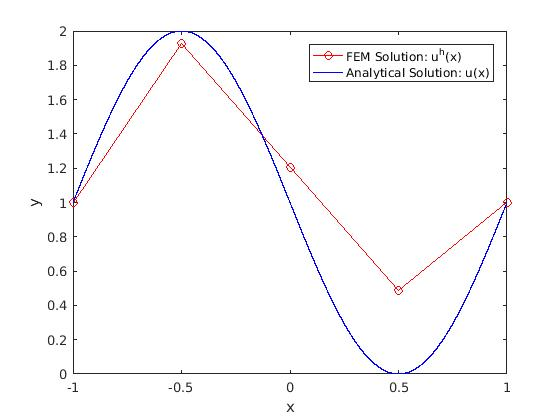
\includegraphics[width=\linewidth]{FEM1DN4.jpg}
  \label{fig:awesome_image1}
\endminipage\hfill
\minipage{0.5\textwidth}
  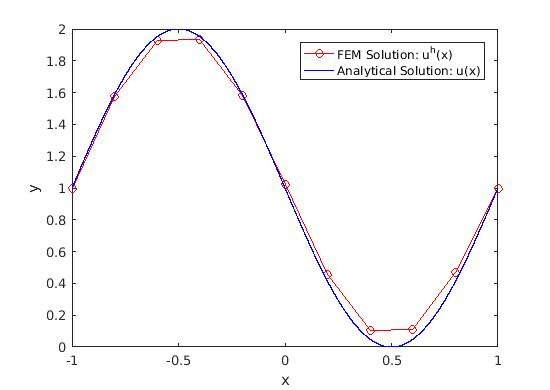
\includegraphics[width=\linewidth]{FEM1DN10.jpg}
  \label{fig:awesome_image2}
\endminipage

\centering
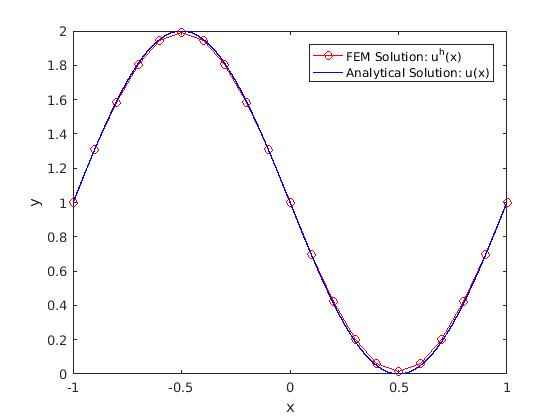
\includegraphics[width=0.5\linewidth]{FEM1DN20.jpg}
\label{fig:awesome_image3}
\caption{Finite Element method solution (red) for $N=4$, $N=10$ and $N=20$ compared with the true solution (blue) $u(x)=1-sin(\pi{x})$}
\end{figure}

\begin{tcolorbox}[title=Task]
By using the example above correct the following FEM code for the solution to the problem 
\begin{equation}\label{BVPc}
\begin{split}
u''(x)&=f(x)\qquad\textnormal{for}\qquad{0}<x<2\\
u(0)&=1\quad{u}(2)=0\\
f(x)&=-x^2
\end{split}
\end{equation}

Copy and paste the following code into a MATLAB script and \textbf{debug} the code. At each stage errors have deliberately included
\end{tcolorbox}
\newpage

\begin{lstlisting}
N = 10;            % Number of piecewise linear elements  
U_L = 1;           % BC at x = 0
U_R = 0;           % BC at x = 2
x = linspace(0,2,N+1)';   % Create set of discrete 
                          % points x_0,x_1,...,x_N
f = x*x;         % The f-vector

A = zeros(N-1,N-1); % Initialise the stiffness and mass matrices
M = zeros(N-1,N+1); % and the g-vector
g = zeros(N,1);
h = diff(x)  % Step length

% Global Matrix Contruction 

A(1,1) = 1/h(1); 
M(1,1) = h(1)/6;
M(1,2) = h(1)/3;
g(1) = U_L/h(1);


A(N-1,N-1)= 1/h(N);
M(N-1,N) = h(N)/6;
M(N-1,N+1)= h(N)/3;
g(N) = U_R/h(N);

% Element matrices without the prefactor h

Ae = [1 -1; -1 1];
Me = [2 1;1 2]/6;

% Loop through elements 2 to N-1
for k = 2:N-1
    A(k-1:k,k-1:k) = A(k-1:k,k-1:k) + Ae/h(k);
    M(k-1:k,k:k+1) = M(k-1:k,k:k+1) + h(k)*Me;
end

% Solve the system of equations
U = [U_L;A\(M*f+g);U_R];   % Solves the system A*U = M*f + g 
                           % with boundary conditions U(-1) = U_L, 
                           %                          U(1) = U_R

% Analytic solution 
t=linspace(-1,1,10000);   % High resolution 
u = 1+t.*(1/6.0)-(t.^4/12.0);

% Plot the solution 
plot(x,U,'ro-');  % Finite Elment Solution 
xlabel('x')
ylabel('y')
hold on          % Plot two functions in the same figure
plot(t,u,'b-')   % Analytic Solution
legend('FEM Solution: u^h(x)','Analytical Solution: u(x)')
    
\end{lstlisting}

\begin{tcolorbox}[title=Task (Difficult)]
Write a code to find the FEM solution to the BVP

\begin{equation}\label{BVPd}
\begin{split}
u''(x)+u(x)&=f(x)\qquad\textnormal{for}\qquad{0}<x<1\\
f(x)&=2e^x
\end{split}
\end{equation}

With boundary conditions 

\begin{equation*}
u(0)=1\qquad{u}(1)=e
\end{equation*}
\end{tcolorbox}

\section*{Danny's Additions}
Throughout this section of the course, we will run through a \textit{mini} project that takes you through the course of developing a solver in MATLAB from start to end, and builds on the skills you have already learnt from this course. The problem we are considering in this case will be a simple problem (you can skip the maths), and we will be creating plots, videos, and a simple GUI (graphical user interface) for this problem.

\subsection*{The Problem}
Consider throwing a ball from some height $h$, at some angle $\alpha$, and at some velocity $v$.\\
\begin{figure}[H]
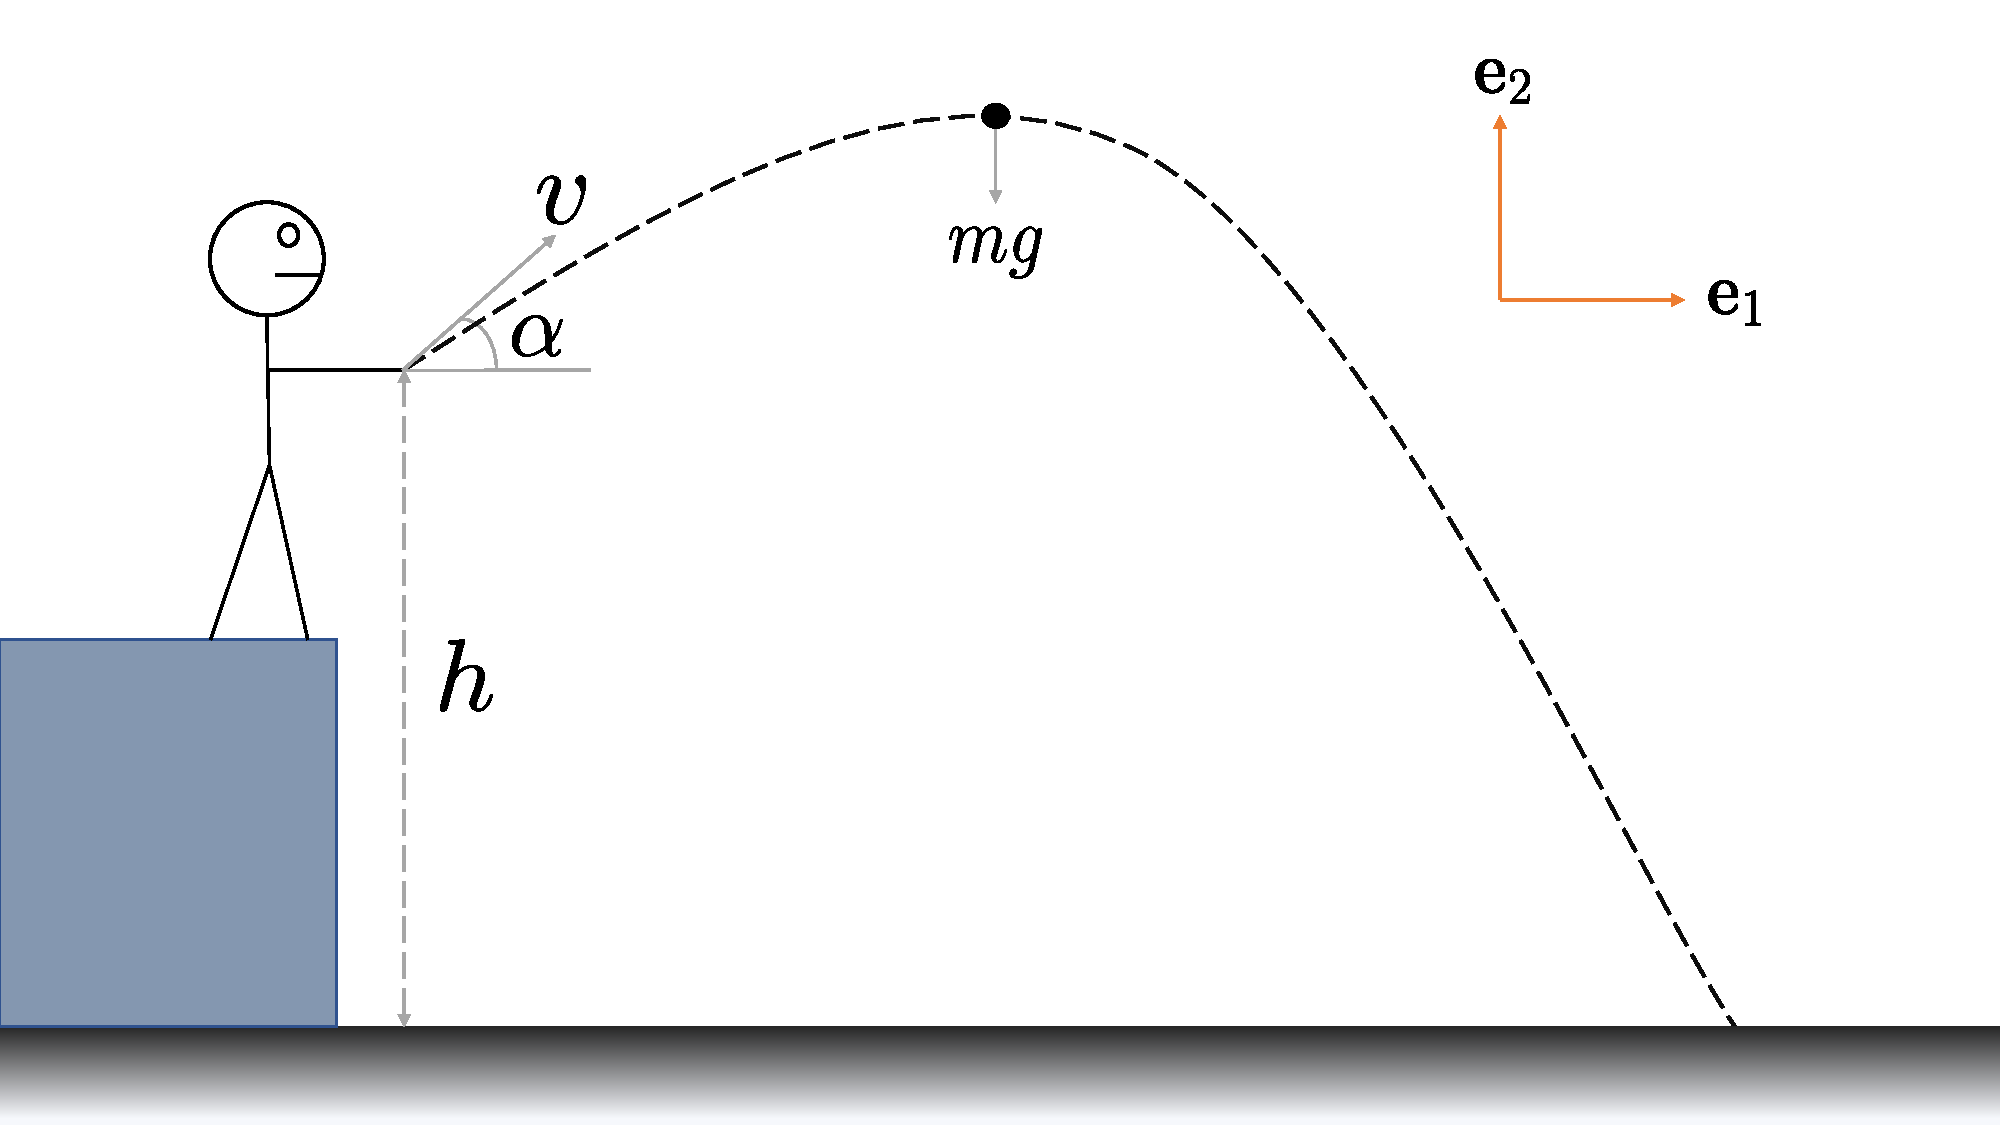
\includegraphics[width = \textwidth]{Projectile.pdf}
\end{figure}
\noindent Assuming no air resistance and using Newton's second law ($F=ma$) we have the following equation of motion for the path of the ball (modelling the ball as a particle)
\begin{equation*}
m\ddot{\*x} = -mg\*e_2,\,\, \text{ s.t }\,\, \*x(0) = h\*e_2, \, \dot{\*x}(0) = v\left(\cos(\alpha)\*e_1+\sin(\alpha)\*e_2\right)
\end{equation*} 
where $\displaystyle \ddot{\*x} = \frac{d^2x}{dt^2}$. Integrating twice and applying the initial conditions yields the answer
\begin{equation*}
\*x = tv\cos(\alpha)\*e_1+\left(-\frac{t^2 g}{2}+tv\sin(\alpha)+h\right)\*e_2,
\end{equation*}
or in the more readable form
\begin{align}
x(t) &= tv\cos(\alpha),\label{EqMot1}\\
y(t) &= -\frac{t^2 g}{2}+tv\sin(\alpha)+h.\label{EqMot2}
\end{align}
The above equations will give the $x$ and $y$ positions through time, and ultimately will be used in MATLAB when we plot the trajectory of the ball. However, to ensure that we plot for the time of flight, we must determine the landing time of the ball. To find this value, we must find the time at which $y = 0$. If $h>0$ we know that $y$ can be zero only once. Alternatively, if the projectile is launched from ground level we have to take the second instance that $y=0$, either way we arrive with the conclusion:
\begin{equation}\label{TimeLand}
t_{\text{land}} = \frac{v\sin(\alpha)+\sqrt{v^2\sin^2(\alpha)+2gh}}{g}.
\end{equation}
We now have all that we need to implement in MATLAB.
\subsection*{Implementation of the Equations}
There are many ways of implementing equations into MATLAB, but we are going to make use of \textbf{Anonymous Functions} to show another way of including functions into your MATLAB scripts. To illustrate the use of an anonymous function, we can use the command line
\begin{lstlisting}
>> f = @(x) x.^2; % To make the function anonymous, use @
>> f(2) % Call on the anonymous function
4
>> f(3) % Try 3^2
9
\end{lstlisting}
We can now begin on implementing the projectile motion equations, and use plotting to visualise the path of the ball.\\
 
\begin{tcolorbox}[title=Task (Moderate)]
Using ProjectileMotion1 inside the tasks folder, modify the script and include the correct equations and insert some initial parameters. Change the parameters, does the graph make physical sense?
\end{tcolorbox}

\begin{tcolorbox}[title=Task (Easy)]
Gravitational acceleration on the moon is given by $g = 1.622ms^{-2}$, change the current script to incorporate this new constant. How do the results change? Is it what you expect?

\tcblower

Extension: Experiment with the values of $g$. What happens if gravity is very weak, or very strong? Is this as you'd expect? Could you use this model to calculate the escape velocity of Earth?

\end{tcolorbox}

\subsection*{Plotting as Time Progresses}
The script ProjectileMotion1 produces a still image of the trajectory of the ball, what if we want to see a movie of how the ball moves through the air as time progresses? Can we do this?\\

\noindent Indeed we can. In fact, we only need to make small modifications to the previous script which includes a plotting over a loop. Below is the loop you will find within script ProjectileMotion2.

\begin{lstlisting}
    for i = 1:length(tspan)
    
        T(i) = tspan(i); % Vector of time steps up to length
        
        % Plot function and include axis labels
        plot(x(T),y(T),'b-','linewidth',1.5)
        xlabel('$x$ distance','interpreter','latex')
        ylabel('$y$ distance','interpreter','latex')
        title('Distance travelled by projectile')
        
        % Set x and y limits to keep axis fixed
        xlim([0 max(x(tspan))]); 
        ylim([0 max(y(tspan))+1]);
        
        drawnow
        
    end
\end{lstlisting}

\noindent In essence, this loop generates a new vector of all time steps included in the first command within the loop. Note that the plotting functions are now different, and include this new vector. This loop then plots the function, draws the graph, and then loops around to include the next time step.\\

\begin{tcolorbox}[title=Task (Moderate)]
The script ProjectileMotion2 contains a completed script that will plot a movie of projectile motion on Earth. The script ProjectileMotion2a plots Earth's projectile, and compares it to the Moon's. The task is to modify ProjectileMotion2a to make it work.
\end{tcolorbox}

\subsection*{Creating a Movie}
Using MATLAB we are able to visualise the projectile motion as a movie, however, what if we'd like to save this movie as an avi file to include in presentations? Fortunately, MATLAB has this capability with its own built in movie maker. However, I have often found in the past that this movie maker can be tricky to use, and produces videos with bad resolution if you follow MATLAB's guide.\\

\noindent The best way to proceed is to print each frame as a separate png file (or other image format), and then use MATLAB's movie maker to combine these into a single avi file. To print the files, the modification is quite simple. First we need to ensure that all frames are the same size, and then we must print the current frame in the loop. The modifications can be seen below (full script is ProjectileMotion3).

\begin{lstlisting}
    ax = axis; % Ensure all images are equal size
    
    for i = 1:length(tspan)
    
        T(i) = tspan(i); % Vector of time steps up to length
        
        % Plot function and include axis labels
        plot(x(T),y(T),'b-','linewidth',1.5)
        xlabel('$x$ distance','interpreter','latex')
        ylabel('$y$ distance','interpreter','latex')
        title('Distance travelled by projectile')
        
        % Set x and y limits to keep axis fixed
        xlim([0 max(x(tspan))]);
        ylim([0 max(y(tspan))+1]);
        
        drawnow
        
        % Print the current frame as a png file
        print(gcf,['Images/' num2str(i,'%0.3d')],'-dpng','-r300') 
        
    end
\end{lstlisting}

\noindent The print command can be modified in a large variety of ways, the important part of this is that the loop now prints the png files into the Images folder. \textbf{You must ensure that there is a folder called Images in your path}. Once the images are printed, you can combine them into a movie by running the MovieMaker script, and the output will be an avi file.\\

\begin{tcolorbox}[title=Task (Optional)]
Use the script ProjectileMotion3 and MovieMaker to create the avi file. Using ProjectileMotion2a, include the print command and the axis command and make a movie from the Earth and Moon comparison.
\end{tcolorbox}

\subsection*{Create a GUI}
While creating a Graphical User Interface (GUI) is non-essential in terms of running MATLAB scripts, it can be a nice way of visualising your scripts and making it more usable for another person. More importantly it can be a way of combining many scripts into one and using them from a simple user interface which reads in options and produces the desired output. This guide is meant to be a quick introduction to GUI creation in MATLAB, and all the code will be supplied.\\

\noindent To create a GUI you can proceed with two routes. The first way is to type \mcode{guide} into the command window which allows you to create a GUI graphically, the second is to create it programatically. There are pros and cons of both, and this is down to personal preference. However I feel that creating a GUI programatically allows for more control and precision over what you create. For this guide, we will create a GUI programatically, however, there are many tutorials for the graphical way on YouTube.\\

\noindent The first step is to create a figure to hold the GUI inside
\begin{lstlisting}
    % This sets up the initial figure to place the GUI inside
    S.f = figure('units','normalized','name',...
    'Projectile Motion Solver','menubar','none',...
    'numbertitle','off','resize','off');
    
    % Set up axis for options
    axOptions = axes('units','normalized','position',[0 0 1 1]);
\end{lstlisting}

\noindent The options within the figure, and axes can be confusing to understand. I find that the best way to gather what they do is to modify them, and see how the GUI changes. The \textbf{key} option is to keep the units \mcode{normalized}, which means that the positions are on a scale of [0,1], i.e. \mcode{[0.5,0.5,0.1,0.2]} places the object in the center, with a width of 0.1, and a height of 0.2. To create entry user controlled buttons, and entry boxes we use the command
\begin{lstlisting}
S.name = uicontrol('style','edit','unit','normalized','position',...
        [0.18,0.85,0.1,0.05],'fontsize',10,'string','2');
\end{lstlisting}
in this case we have created an edit box, where a user can input data which will be read into the solver (the initial value here is 2). You can create other ui controls, for example:
\begin{itemize}
\item \mcode{'style','slider'} - slider bar
\item \mcode{'style','pop'} - creates a drop down menu
\item \mcode{'style','pushbutton'} - creates a push button to run scripts
\item \mcode{'style','check'} - creates a checkbox
\item And many others!
\end{itemize}
Including all the ui controls can be fiddly, and usually takes time to place them correctly. However, once they are placed they are effectively useless unless you call on their values correctly. As an illustration the script ProjectileGUI implements these ui controls to plot the motion of a projectile using the previous scripts. The key element of this script is the run button, which is created by
\begin{lstlisting}
    % Run code
    S.Run = uicontrol('style','pushbutton','unit','normalized',...
    'position',[0.075,0.45,0.15,0.05],'fontsize',10,'string',...
    'Run','callback',{@Run,S});
\end{lstlisting}
Notice that this has a callback, which basically means that once the button is pressed a function called Run is activated, and is fed in all the data through \mcode{S}. Below is half of the Run function
\begin{lstlisting}
function [] = Run(varargin)
    S = varargin{3}; % Reads the list
    
    % Get values for projectile motion
    alpha = get(S.Angle,'val'); % Obtain angle from slider bar
    h = str2double(get(S.Height,'string')); % Convert string to number
    v = str2double(get(S.Velocity,'string')); % Get velocity
...
\end{lstlisting}
this function when used will read in all values using the list \mcode{S}, which is why we have named things \mcode{S.Name}. Once the list is read, we obtain the value by using \mcode{str2double(get(S.Name,'string'));}, which takes the string from the box and converts it to a number for MATLAB to use. \textbf{Note}: this may change if you assign the edit box a numerical value instead of a string, or if you use a checkbox where the output is binary.\\

\begin{tcolorbox}[title=Task (Optional)]
Using ProjectileGUI as an example, add in another box which controls variable gravity. i.e. create an edit box where you can choose the strength of gravity which is read in by the solver (solution given).
\end{tcolorbox}

\end{document}